\subsubsection{Sample Dimensions}
\noindent Three timber lap joint  sample were tested on 26 February 2026 using the Machine at ITC lab. The samples are the stepped lap joint geometry. The shear plane area $A$ is defined as the width $b$ multiplied by the shear height $h^{\prime}$.

\begin{table}[H]
\centering
\begin{tabular}{CCCCC}
\hline
No. & $a (mm)$ & $b (mm)$ & $h(mm)$& $h^\prime + h (mm)$\\ \hline
1  & 20.03 & 29.95 & 16.18 & 28.03 \\
2  & 20.18& 30.66 & 16.65 & 28.14 \\
3  & 20.09& 29.92 & 16.29 & 28.00\\\hline
\end{tabular}
\caption{Dimension of Sample}
\end{table}
\begin{figure}[H]
\centering
\begin{minipage}{0.4\textwidth}
\centering
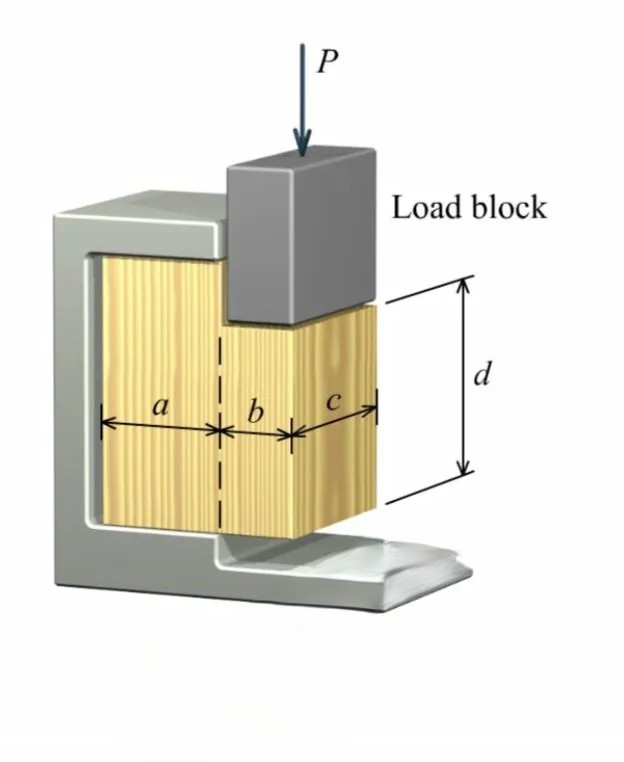
\includegraphics[width=\linewidth]{sample4/image/sampledimension.jpg}
\end{minipage}
\begin{minipage}{0.40\textwidth}
\centering
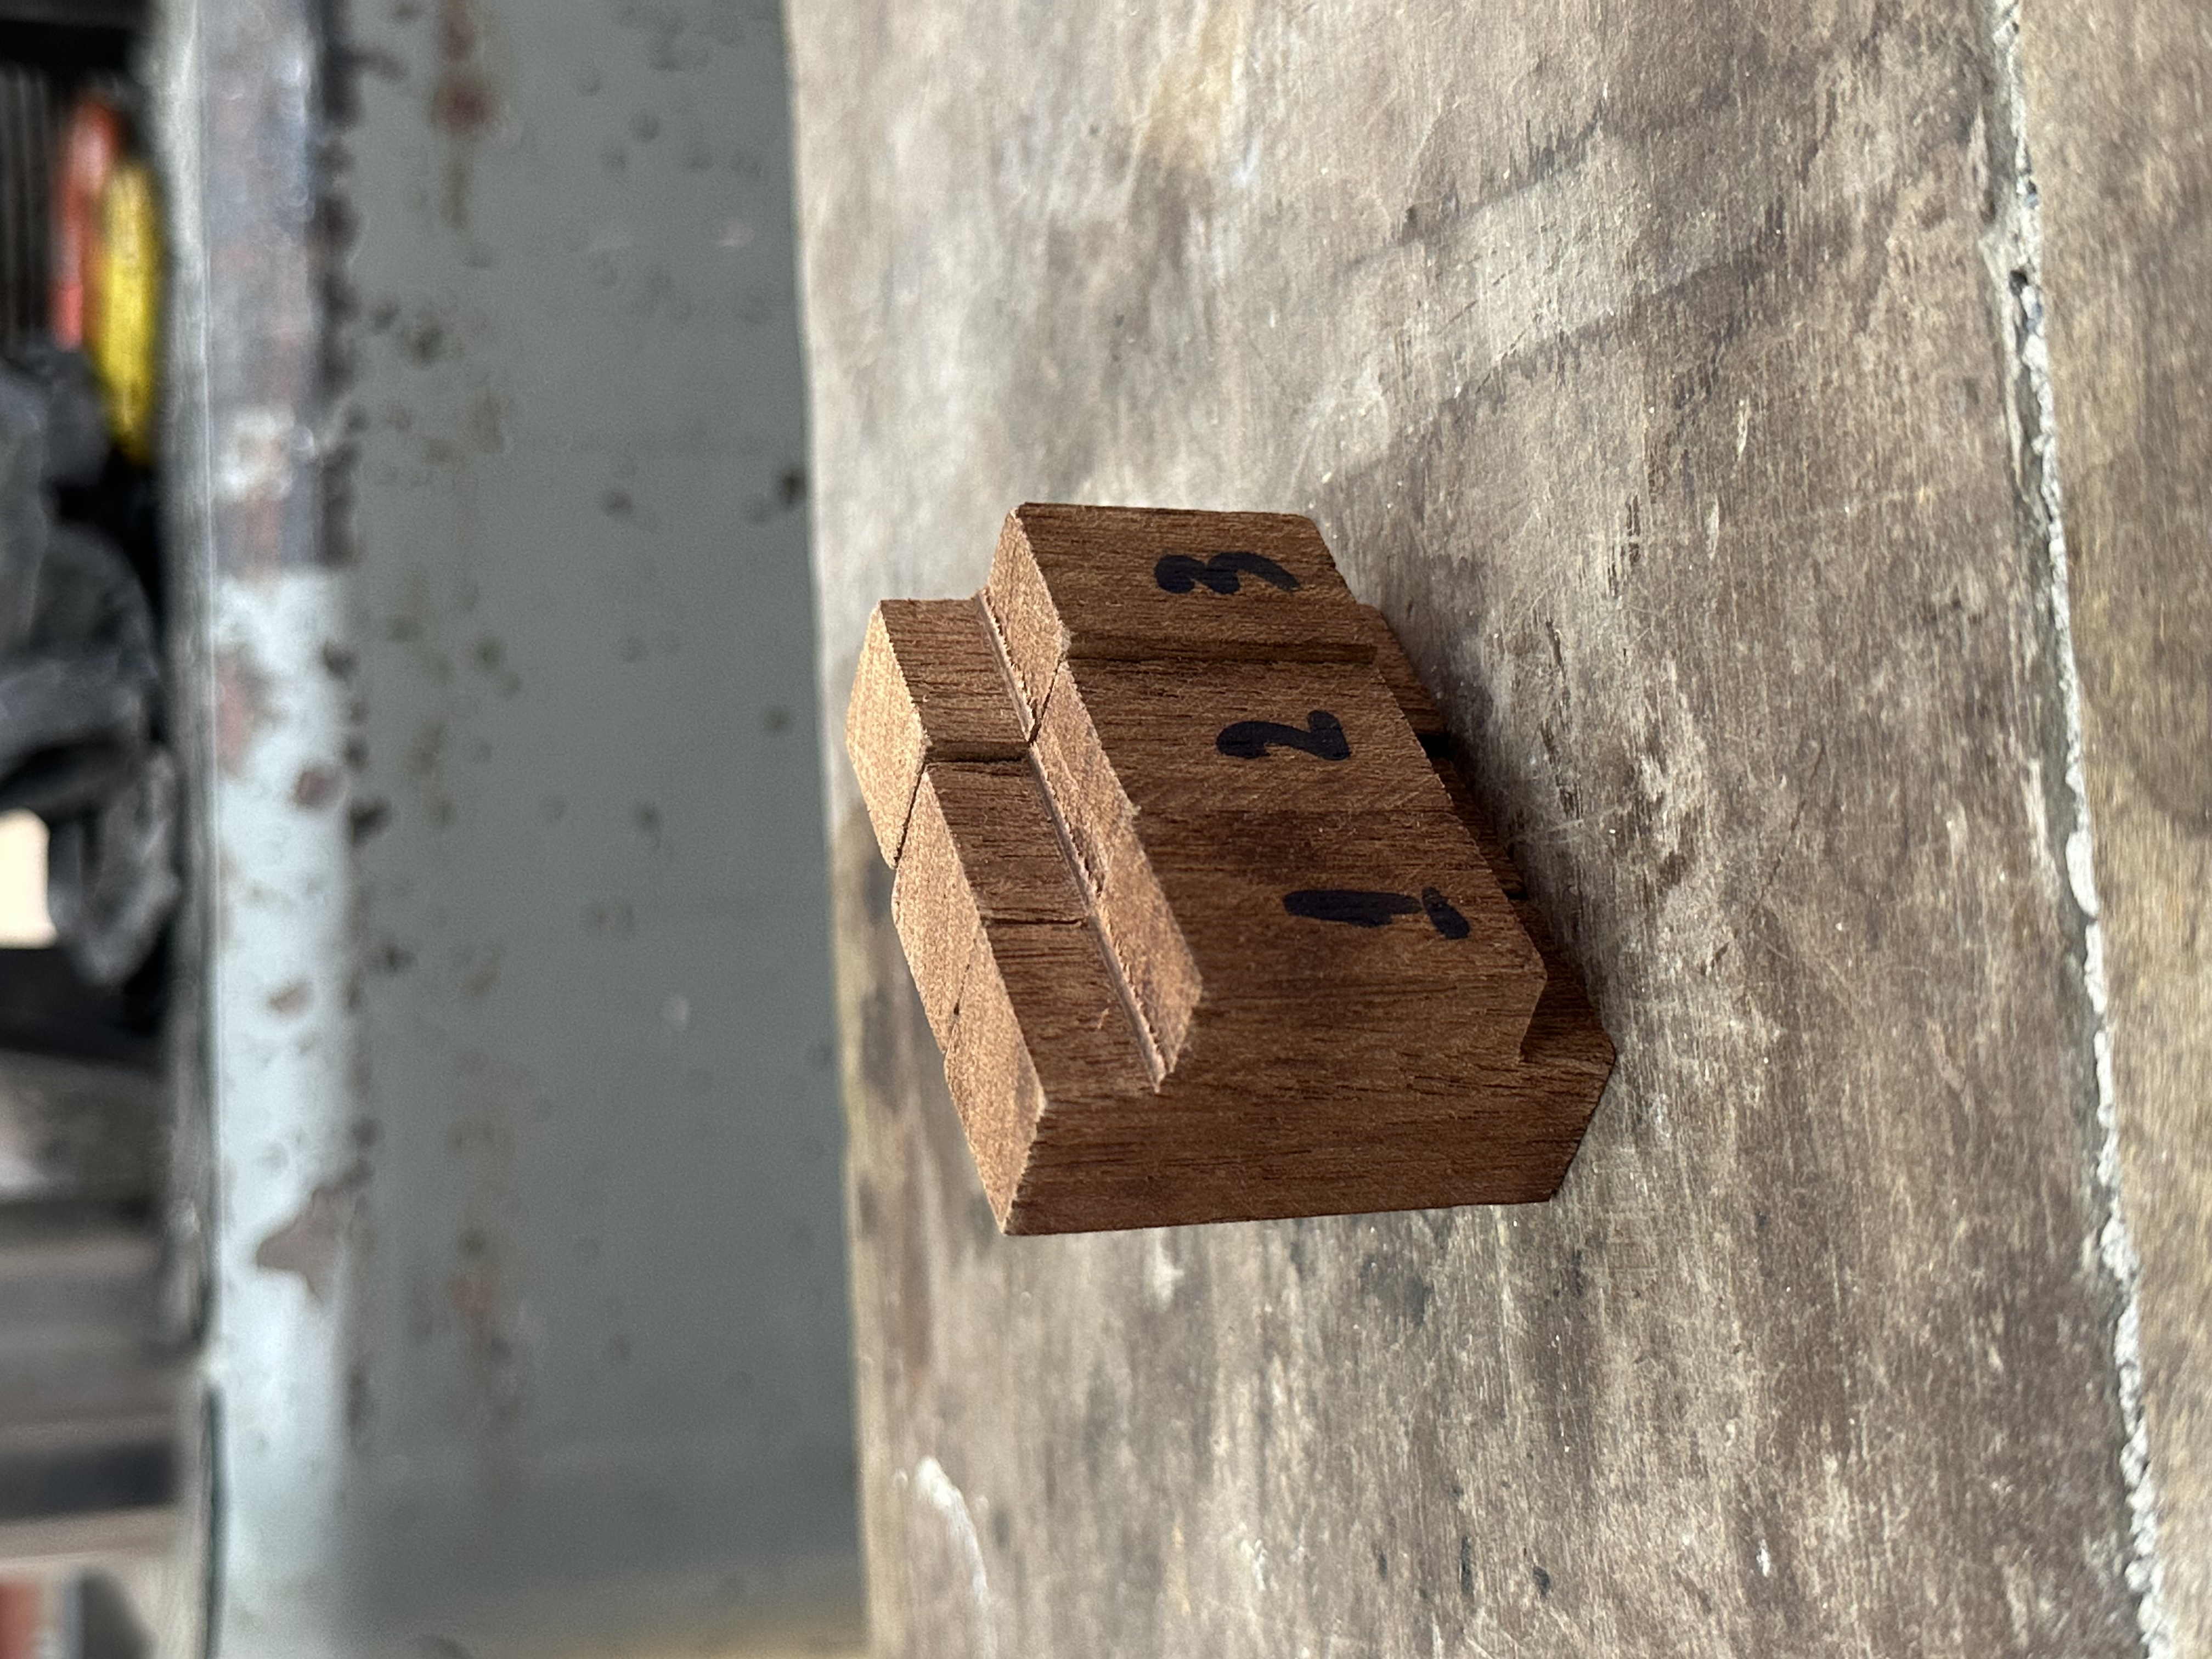
\includegraphics[width=\linewidth,angle=-90]{sample4/image/sheartestsample.JPG}
\end{minipage}
\caption{Shear testing's sample}
\end{figure}
